%
% operation.tex -- Gruppen-Operation auf einer elliptischen Kurve
%
% (c) 2021 Prof Dr Andreas Müller, OST Ostschweizer Fachhochschule
%
\bgroup
\begin{frame}[t]
\setlength{\abovedisplayskip}{5pt}
\setlength{\belowdisplayskip}{5pt}
\frametitle{Gruppenoperation}
\vspace{-20pt}
\begin{columns}[t,onlytextwidth]
\begin{column}{0.40\textwidth}
\begin{center}
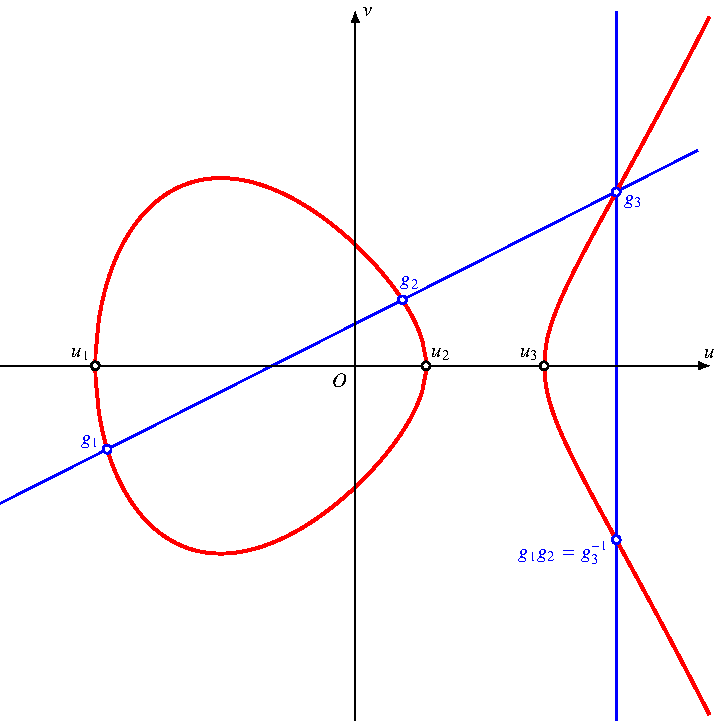
\includegraphics[width=\textwidth]{../../buch/chapters/90-crypto/images/elliptic.pdf}
\end{center}
\vspace{-23pt}
\uncover<8->{%
\begin{block}{Verifizieren}
\begin{enumerate}
\item<9-> Assoziativ?
\item<10-> Neutrales Element $\mathstrut=\infty$
\item<11-> Involution = Inverse?
\end{enumerate}
\end{block}}
\end{column}
\begin{column}{0.56\textwidth}
\begin{block}{Gerade}
$g_1,g_2\in G$, $t\in \Bbbk$
\begin{align*}
g(t)
&=
tg_1+(1-t)g_2
\\
\uncover<2->{
\begin{pmatrix}X(t)\\Y(t)\end{pmatrix}
&=
t\begin{pmatrix}x_1\\y_1\end{pmatrix}
+
(1-t)\begin{pmatrix}x_2\\y_2\end{pmatrix}
\in\Bbbk^2
}
\end{align*}
\end{block}
\vspace{-13pt}
\uncover<3->{%
\begin{block}{3. Schnittpunkt}
$g(t)$ einsetzen in die elliptische Kurve
\[
p(t)
=
Y(t)^2+X(t)Y(t)-X(t)^3-aX(t)-b=0
\]
\vspace{-12pt}
\begin{enumerate}
\item<4->
kubisches Polynom mit Nullstellen $t=0,1$
\item<5->
$p(t) $ ist durch $t(t-1)$ teilbar
\item<6->
$p(t) = t(t-1)(Jt+K)=0
\uncover<7->{\Rightarrow t=-K/J$}
\end{enumerate}
\end{block}}
\end{column}
\end{columns}
\end{frame}
\egroup
